Um Informationen bzw. Bits zu manipulieren, werden Schaltungen ben\"otigt welche Gatter beinhalten. Dies gilt f\"ur klassische Rechner und Quantencomputer. Um in der Digitaltechnik die Funktionsweise von Gattern darzustellen werden gerne Wahrheitstabellen genutzt (rechte Spalte Tabelle \ref{table:Qubit-Gatter}). Bekannte Gatter-Typen aus der Digitaltechnik, wie der Negation oder dem Exklusiv-ODER k\"onnen auch in der Welt der Quantencomputer abgebildet werden. Jedoch ist der Aufbau dieser Gatter etwas gew\"ohnungsbed\"urfdig, denn die Realisierung eines auf $n$ Qubits operierenden Gatters erfolgt durch eine unit\"are $2^{n}\times 2^{n}$-Matrix. Die Anwendung eines Gatters auf einen Zustandvektor entspricht mathematisch also einer unit\"aren Transformation und f\"uhrt eine Rotation auf der Bloch-Kugel aus. Dies geschieht durch die Bildung des Skalarprodukts \"uber der unit\"aren Matrix und dem Zustandvektor. \\ \\
Eine Matrix wird als unit\"ar bezeichnet, wenn das Produkt aus dieser Matrix und dessen adjungierte Matrix eine Einheitsmatrix bildet.
\begin{equation}
  I = A^{\dagger} A
\end{equation}
Die Adjungierte Matrix wird gebildet, indem alle Eintr\"age in dieser Matrix komplex konjungiert und transponiert werden.
\begin{equation}
  A^{\dagger} = A^{*T}
\end{equation}
Somit sind alle Quantengatter unit\"are Matrizen, genau wie die drei aus der Quantenmechnik bekannten Paulimatrizen $X, Y$ und $Z$ Tabelle \ref{table:Qubit-Gatter}. Diese f\"uhren eine Rotation von $\pi$ um die $x, y$ und $z$-Achse auf der Bloch-Kugel durch. Das Hadamard-Gatter $H$ erm\"oglicht eine Abweichung der Basiszust\"ande $|0\rangle$ und $|1\rangle$ und erzeugt eine Superposition dieser Zust\"ande \cite{Qiskit-Textbook}.
Dies w\"aren die Zustandvektoren $|+\rangle$ und $|-\rangle$, welche auch auf der Bloch-Kugel in Abbildung \ref{fig:Bloch-Kugel} zu erkennen sind. \\ \\
Zwei parametrisierte Gatter, das $P$-Gatter (Phasen-Gatter) und $U$-Gatter die nicht in Tabelle \ref{table:Qubit-Gatter} aufgef\"uhrt sind, erlauben die Spezifizierung von s\"amtlichen Gattern bzw. unedlich vielen Gattern die auf einem Qubit operieren.
\begin{equation}
\begin{aligned}
P(\phi) &= \begin{bmatrix}1 & 0 \\ 0 & e^{i\phi} \end{bmatrix} &&\qquad \phi \in \mathbf{R}\\[1em]
U(\theta, \phi, \lambda) &= \begin{bmatrix} \cos\left(\frac{\theta}{2}\right) & -e^{i\lambda}sin\left(\frac{\theta}{2}\right) \\
e^{i\phi}sin\left(\frac{\theta}{2}\right) & e^{i(\phi+\lambda)}sin\left(\frac{\theta}{2}\right)
\end{bmatrix} &&\qquad \theta, \phi, \lambda \in \mathbf{R}
\end{aligned}
\end{equation}

\vspace{1.2cm}
%%%%%%%%%%%%%%%%%%%%%%%Table%%%%%%%%%%%%%%%%%%%%%%%%%%%%%%%%

\begin{table}[h] 
\begin{tabular}{@{\hspace{0.7cm}}c@{\hspace{0.7cm}} | @{\hspace{0.7cm}}c@{\hspace{0.7cm}} | @{\hspace{0.8cm}}c@{\hspace{0.7cm}}}
\hline 
Matrix & Schaltungssymbol & Wahrheitstabelle \\
\hline & \\
$X = \begin{bmatrix} 0 & 1 \\ 1 & 0 \end{bmatrix}$ &
\raisebox{-.3\height}{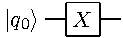
\includegraphics[width=0.2\textwidth]{figures/pauli_x.pdf}} &
\begin{tabular}{|c||c||c|}
\hline
Fall & $|q\rangle$ & $X|q\rangle$ \\
\hline \hline 
1 & $|0\rangle$ & $|1\rangle$ \\
2 & $|1\rangle$ & $|0\rangle$ \\
\hline
\end{tabular} \\&\\

%%%%%%%%%%%%%%%%%%%%%%%%%%%%%%%%%%%%%%%%%%%%%%%%%%%%%%%%%%%%%%

$Y = \begin{bmatrix} 0 & -i \\ i & 0 \end{bmatrix}$ &
\raisebox{-.3\height}{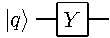
\includegraphics[width=0.2\textwidth]{figures/pauli_y.pdf}} &
\begin{tabular}{|c||c||c|}
\hline
Fall & $|q\rangle$ & $Y|q\rangle$ \\
\hline \hline 
1 & $|0\rangle$ & $i|1\rangle$ \\
2 & $|1\rangle$ & $-i|0\rangle$ \\
\hline
\end{tabular} \\&\\

%%%%%%%%%%%%%%%%%%%%%%%%%%%%%%%%%%%%%%%%%%%%%%%%%%%%%%%%%%%%%%

$Z = \begin{bmatrix} 1 & 0 \\ 0 & -1 \end{bmatrix}$ &
\raisebox{-.3\height}{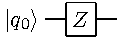
\includegraphics[width=0.2\textwidth]{figures/pauli_z.pdf}} &
\begin{tabular}{|c||c||c|}
\hline
Fall & $|q\rangle$ & $Z|q\rangle$ \\
\hline \hline 
1 & $|0\rangle$ & $|0\rangle$ \\
2 & $|1\rangle$ & $-|1\rangle$ \\
\hline
\end{tabular} \\&\\

%%%%%%%%%%%%%%%%%%%%%%%%%%%%%%%%%%%%%%%%%%%%%%%%%%%%%%%%%%%%%%

$H = \frac{1}{\sqrt{2}} \begin{bmatrix} 1 & 1 \\ 1 & -1 \end{bmatrix}$ &
\raisebox{-.3\height}{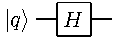
\includegraphics[width=0.2\textwidth]{figures/hadamard.pdf}} &
\begin{tabular}{|c||c||c|}
\hline
Fall & $|q\rangle$ & $H|q\rangle$ \\
\hline \hline 
1 & $|0\rangle$ & $\frac{|0\rangle+|0\rangle}{\sqrt{2}}$ \\
2 & $|1\rangle$ & $\frac{|0\rangle-|1\rangle}{\sqrt{2}}$ \\
\hline
\end{tabular} \\&\\

%%%%%%%%%%%%%%%%%%%%%%%%%%%%%%%%%%%%%%%%%%%%%%%%%%%%%%%%%%%%%%

$S = \begin{bmatrix} 1 & 0 \\ 0 & i \end{bmatrix}$ &
\raisebox{-.3\height}{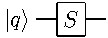
\includegraphics[width=0.2\textwidth]{figures/phase.pdf}} &
\begin{tabular}{|c||c||c|}
\hline
Fall & $|q\rangle$ & $S|q\rangle$ \\
\hline \hline 
1 & $|0\rangle$ & $|0\rangle$ \\
2 & $|1\rangle$ & $i|1\rangle$ \\
\hline
\end{tabular} \\&\\

%%%%%%%%%%%%%%%%%%%%%%%%%%%%%%%%%%%%%%%%%%%%%%%%%%%%%%%%%%%%%%

$T = \begin{bmatrix} 1 & 0 \\ 0 & e^{i\frac{\pi}{4}} \end{bmatrix}$ &
\raisebox{-.3\height}{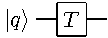
\includegraphics[width=0.2\textwidth]{figures/t_dagger.pdf}} &
\begin{tabular}{|c||c||c|}
\hline
Fall & $|q\rangle$ & $T|q\rangle$ \\
\hline \hline 
1 & $|0\rangle$ & $|0\rangle$ \\
2 & $|1\rangle$ & $e^{i\frac{\pi}{4}} |1\rangle$ \\
\hline
\end{tabular} \\&\\
\hline
\end{tabular}
\caption{Grundlegende 1-Qubit Gatter}
\label{table:Qubit-Gatter}
\end{table}
Aus dem $P$-Gatter lassen sich die Gatter $Z, S$ und $T$ konstruieren. \ref{eqn:konstruktion} zeigt die Spezifizierung des $S$- und $T$-Gattes durch das Phasengatter.
\begin{equation}\label{eqn:konstruktion}
P\left(\phi=\frac{\pi}{2}\right) = S \qquad P(\phi=\pi) = Z .
\end{equation}
Das $U$-Gatter erm\"oglicht die Spezifizierung jeglicher Gatter, z.B. kann das Hadamard-Gatter folgenderma\ss en durch das $U$-Gatter spezifiziert werden
\begin{equation}
U\left(\theta= \frac{\pi}{2}, \phi=0, \lambda=\pi\right) = H .
\end{equation}
Somit kann es eine gro\ss e Menge an n\"utzlichen Gattern geben, die auf einem Qubit operieren. Es ist m\"oglich diese Gatter auch auf meheren Qubits operieren zu lassen. Diese Gatter werden dann kontrollierte Gatter gennant, da diese ein oder mehrere kontrollierende Qubits \textit{(controlled qubits)} und ein Zielqubit \textit{(target qubit)} beinhalten. Tabelle \ref{table:2Qubit-Gatter} zeigt oft genutzte Gatter die auf mehr als einem Qubit operieren.\\\\ Ein kontrolliertes Gatter funktioniert folgenderma\ss en: Immer dann wenn sich die kontrolliernden Bits im Zustand 1 befinden wird eine Transformation auf das Zielbit ausgef\"uhrt.
Die meisten dieser kontrollierten Gatter k\"onnen durch 1-Qubit Gatter und dem kontrollierten $X$-Gatter \textit{(CNOT o. CX)} rekonstruiert werden \cite{Barenco_1995}. Das hei\ss t auch, das alle in Tabelle \ref{table:2Qubit-Gatter} dargestellten Gatter, die selbe unit\"are Transformation wie die Gatter aus Tabelle \ref{table:Qubit-Gatter} ausf\"uhren. Diesmal jedoch nur auf das Zielbit, immer genau dann wenn das kontrollierende Bit 1 ist. \\\\
Bei dem Aufbau einer Quantenschaltung ist es somit wichtig zu wissen, welches Qubit als kontrolliertes Bit und welches als Zielbit f\"ur ein Gatter dient. Aus diesem Grund erhalten in dieser Ausarbeitung die kontrollierten Gatter einen Index. In diesem stellen die ersten Zahlen die kontrollierenden Bits und die letzte Zahl das Zielbit dar. \ref{eqn:zerlegung} zeigt die Zusammensetzung der beiden m\"oglichen Matrizen f\"ur das $CX$-Gatter.
\begin{equation}\label{eqn:zerlegung}
\begin{aligned}
CX_{01} = |0\rangle\langle0|\otimes I +|1\rangle\langle1|\otimes X \\
CX_{10} = I \otimes |0\rangle\langle0|+X \otimes|1\rangle\langle1|
\end{aligned}
\end{equation}
Dabei ist $|x\rangle\langle x|$ das \"au\ss ere Produkt. $\langle x|$ ist der komplex konjungiert und transponiert Vektor von $|x\rangle$ und $I$ die Einheitsmatrix.\\
Ein wichtiges Gatter in Tabelle \ref{table:2Qubit-Gatter} ist das $SWAP$-Gatter, welches die Funktion erf\"ullt die Zust\"ande der beiden Qubits zu tauschen. Auch dieses Gatter kann z.B. nur durch CX-Gatter aufgebaut werden \ref{fig:cnot2swap} (vgl. \cite{Qiskit-Textbook}).
\begin{figure}[h]
\centering
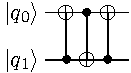
\includegraphics[width=0.28\textwidth]{figures/cnot2swap.pdf}
\caption{$SWAP$-Gatter realisiert aus 3 kontrollierten $CX$-Gattern}
\label{fig:cnot2swap}
\end{figure}
Jeodch ist dies nicht der einzige Weg ein SWAP-Gatter aus anderen Gattern zu realisieren.
%%%%%%%%%%%%%%%%%%%%%%%Table Multi%%%%%%%%%%%%%%%%%%%%%%%%%%%%%%%%

\begin{table}[h]
\hspace{-1cm}
\begin{tabular}{c|c|c}
\hline 
Matrix & Schaltungssymbol & Wahrheitstabelle \\
\hline & \\
$CX_{01} = \begin{bmatrix} 1 & 0 & 0 & 0 \\ 0 & 1 & 0 & 0 \\ 0 & 0 & 0 & 1 \\ 0 & 0 & 1 & 0 \end{bmatrix}$ &
\raisebox{-.5\height}{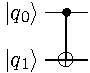
\includegraphics[width=0.16\textwidth]{figures/cnot.pdf}} &
\begin{tabular}{|c||c||c|}
\hline
Fall & $|q_0 q_1\rangle$ & $CX_{01}|q_0 q_1\rangle$ \\
\hline \hline 
1 & $|00\rangle$ & $|00\rangle$ \\
2 & $|01\rangle$ & $|01\rangle$ \\
3 & $|10\rangle$ & $|11\rangle$ \\
4 & $|11\rangle$ & $|10\rangle$ \\
\hline
\end{tabular} \\&\\

%%%%%%%%%%%%%%%%%%%%%%%%%%%%%%%%%%%%%%%%%%%%%%%%%%%%%%%%%%%%%%

$CZ_{01} = \begin{bmatrix} 1 & 0 & 0 & 0 \\ 0 & 1 & 0 & 0 \\ 0 & 0 & 1 & 0 \\ 0 & 0 & 0 & -1 \end{bmatrix}$ &
\raisebox{-.5\height}{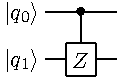
\includegraphics[width=0.2\textwidth]{figures/cz.pdf}} &
\begin{tabular}{|c||c||c|}
\hline
Fall & $|q_0 q_1\rangle$ & $CZ_{01}|q_0 q_1\rangle$ \\
\hline \hline 
1 & $|00\rangle$ & $|00\rangle$ \\
2 & $|01\rangle$ & $|01\rangle$ \\
3 & $|10\rangle$ & $|10\rangle$ \\
4 & $|11\rangle$ & $-|11\rangle$ \\
\hline
\end{tabular} \\&\\

%%%%%%%%%%%%%%%%%%%%%%%%%%%%%%%%%%%%%%%%%%%%%%%%%%%%%%%%%%%%%%

$SWAP = \begin{bmatrix} 1 & 0 & 0 & 0 \\ 0 & 0 & 1 & 0 \\ 0 & 1 & 0 & 0 \\ 0 & 0 & 0 & 1 \end{bmatrix}$ &
\raisebox{-.5\height}{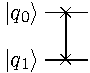
\includegraphics[width=0.16\textwidth]{figures/swap.pdf}} &
\begin{tabular}{|c||c||c|}
\hline
Fall & $|q_0 q_1\rangle$ & $SWAP|q_0 q_1\rangle$ \\
\hline \hline 
1 & $|00\rangle$ & $|00\rangle$ \\
2 & $|01\rangle$ & $|10\rangle$ \\
3 & $|10\rangle$ & $|01\rangle$ \\
4 & $|11\rangle$ & $|11\rangle$ \\
\hline
\end{tabular} \\&\\

%%%%%%%%%%%%%%%%%%%%%%%%%%%%%%%%%%%%%%%%%%%%%%%%%%%%%%%%%%%%%%

$CCX_{012} = \begin{bmatrix} I_2 & 0_2 & 0_2 & 0_2 \\ 0_2 & I_2 & 0_2 & 0_2 \\ 0_2 & 0_2 & I_2 & 0_2 \\ 0_2 & 0_2 & 0_2 & X \end{bmatrix}$ &
\raisebox{-.5\height}{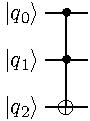
\includegraphics[width=0.16\textwidth]{figures/toffoli.pdf}} &
\begin{tabular}{|c||c||c|}
\hline
Fall & $|q_0 q_1 q_2 \rangle$ & $CCX_{012}|q_0 q_1 q_2\rangle$ \\
\hline \hline 
1 & $|000\rangle$ & $|000\rangle$ \\
2 & $|001\rangle$ & $|001\rangle$ \\
3 & $|010\rangle$ & $|010\rangle$ \\
4 & $|011\rangle$ & $|011\rangle$ \\
5 & $|100\rangle$ & $|100\rangle$ \\
6 & $|101\rangle$ & $|101\rangle$ \\
7 & $|110\rangle$ & $|111\rangle$ \\
8 & $|111\rangle$ & $|110\rangle$ \\
\hline
\end{tabular} \\&\\

%%%%%%%%%%%%%%%%%%%%%%%%%%%%%%%%%%%%%%%%%%%%%%%%%%%%%%%%%%%%%%

$CP_{10} = \begin{bmatrix} 1 & 0 & 0 & 0 \\ 0 & 1 & 0 & 0 \\ 0 & 0 & 1 & 0 \\ 0 & 0 & 0 & e^{i\phi} \end{bmatrix}$ &
\raisebox{-.5\height}{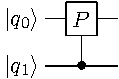
\includegraphics[width=0.2\textwidth]{figures/cp.pdf}} &
\begin{tabular}{|c||c||c|}
\hline
Fall & $|q_0 q_1\rangle$ & $CP_{10}|q_0 q_1\rangle$ \\
\hline \hline 
1 & $|00\rangle$ & $|00\rangle$ \\
2 & $|01\rangle$ & $|01\rangle$ \\
3 & $|10\rangle$ & $|10\rangle$ \\
4 & $|11\rangle$ & $e^{i\phi}|11\rangle$ \\
\hline
\end{tabular} \\&\\
\hline
\end{tabular}
\caption{Ausgew\"ahlte 2-, 3-Quanten Gatter}
\label{table:2Qubit-Gatter}
\end{table}
\clearpage
